\chapter{The Thorin Framework for Automorphic L Functions}\label{ch:10b}

Thorin introduced generalized gamma convolutions in 1977 to prove that the Pareto and lognormal laws are infinitely divisible \cite{thorin1977,thorin1977b}. Much later they were proposed as a language for the reciprocal of Riemann's $\Xi$ function \cite{polson2017}. In \cite{polson2018vdp} the first author proved, for real entire functions of order at most one in the Laguerre P\'olya setting, that all zeros lie on the critical axis if and only if Thorin's condition holds, identified the Thorin measure as $\sum_k\delta_{\gamma_k^2}$, and recast the Hadamard factorisation as a van Dantzig pair and a Wald couple (Chapter~\ref{ch:10d}), with applications to $\xi$, Dirichlet and modular $L$ functions and the Dedekind $\eta$ function. Chapter~\ref{ch:10} built that dictionary for the discriminant form $\Delta$; this chapter shows that nothing in it is special to $\Delta$. For every cuspidal automorphic representation $\pi$ of $\GL_n$ over $\Q$ we build an even completion $\Xi_\pi$ of $\Lambda(s,\pi)$, real and nonnegative on the real axis, and prove that the generalized Riemann hypothesis for $\pi$ is equivalent to each of six positivity statements: a Thorin representation, complete monotonicity of a L\'evy function, a Stieltjes property, a Herglotz inequality, a Stieltjes moment property of power sums computable from central Taylor coefficients alone, and, when the P\'olya kernel is positive, a moment property of the even cumulants of the P\'olya variable. We then relax the Thorin property into parabolic conditions, recover de Bruijn's bound as the unconditional case, read the order of central vanishing as a degenerate Thorin atom, test the criteria numerically on eleven $L$ functions, and locate the boundary of the framework at the Selberg zeta function. All of it is reformulation; none of it proves a Riemann hypothesis.

\section{Thorin, Stieltjes and Bernstein}

We use the definition of a generalized gamma convolution (GGC) and its Thorin measure from Definition~\ref{def:ch10ggc}: a law on $[0,\infty)$ whose Laplace transform is
\begin{equation}\label{eq:10bggc}
\varphi(s) = \exp\Bigl(-as-\int_{(0,\infty)}\log\Bigl(1+\frac st\Bigr)\tau(dt)\Bigr),\qquad s\ge0,
\end{equation}
with drift $a\ge0$ and Thorin measure $\tau\ge0$ subject to the integrability conditions stated there \cite{thorin1977,bondesson1992}. The analytic fact behind every equivalence below is Lemma~\ref{lem:ch10nonvanish}: $\varphi$ extends to a holomorphic function on $\C\setminus(-\infty,0]$ \emph{without zeros}. Three classical theorems complete the toolkit.\index{generalized gamma convolution}

\begin{theorem}[Bernstein]\label{thm:10bbernstein}
A function $f$ on $(0,\infty)$ is completely monotone, that is $(-1)^mf^{(m)}\ge0$ for all $m$, if and only if $f(x) = \int e^{-tx}\mu(dt)$ for a unique positive measure $\mu$ on $[0,\infty)$.
\end{theorem}

\begin{definition}\label{def:10bstieltjes}
A \emph{Stieltjes function}\index{Stieltjes function} is a function $g:(0,\infty)\to[0,\infty)$ of the form
\[
g(s) = \frac as + b + \int_{(0,\infty)}\frac{\sigma(dt)}{s+t},\qquad a,b\ge0,\quad \int_{(0,\infty)}\frac{\sigma(dt)}{1+t}<\infty .
\]
\end{definition}

Differentiating \eqref{eq:10bggc} gives $-\varphi'/\varphi = a+\int\tau(dt)/(s+t)$, so minus the logarithmic derivative of a GGC transform is a Stieltjes function with no pole at the origin; conversely a Stieltjes function $g$ with $a=0$ and $\int_0^1g(u)\,du<\infty$ integrates to a GGC transform $\exp(-\int_0^sg)$, with drift $b$ and Thorin measure $\sigma$. The integral part is the Laplace transform of a completely monotone function, $\int\sigma(dt)/(s+t) = \int_0^\infty e^{-sx}\int e^{-tx}\sigma(dt)\,dx$, and Stieltjes functions have a classical complex analytic description.

\begin{theorem}[Nevanlinna Pick characterisation]\label{thm:10bpick}
A function $g:(0,\infty)\to[0,\infty)$ is a Stieltjes function if and only if it extends holomorphically to $\C\setminus(-\infty,0]$ and satisfies $\operatorname{Im}g(s)\le0$ whenever $\operatorname{Im}s>0$.
\end{theorem}

The direction from the representation to the extension is elementary: for $s$ in a compact $K\subset\C\setminus(-\infty,0]$ the continuous positive function $(s,t)\mapsto|s+t|/(1+t)$ on $K\times[0,\infty]$ is bounded below by some $c_K>0$, so the integral converges locally uniformly, and $\operatorname{Im}(s+t)^{-1} = -\operatorname{Im}s/|s+t|^2\le0$. The converse rests on the Herglotz representation \cite{schillingsongvondracek2012}; we need only the elementary direction.\index{Herglotz function}

\begin{theorem}[Stieltjes]\label{thm:10bstieltjesmoment}
A real sequence $(m_j)_{j\ge0}$ is a Stieltjes moment sequence, $m_j = \int_{[0,\infty)}u^j\nu(du)$ for a positive measure $\nu$ on $[0,\infty)$, if and only if the Hankel matrices $(m_{i+j})_{i,j=0}^N$ and $(m_{i+j+1})_{i,j=0}^N$ are positive semidefinite for every $N\ge0$.
\end{theorem}

Necessity is the identity $\sum c_ic_jm_{i+j+\ell} = \int u^\ell(\sum c_iu^i)^2\nu(du)$ for $\ell=0,1$; sufficiency is Stieltjes' theorem \cite{stieltjes1894,akhiezer1965}.\index{Stieltjes moment problem}

\section{The self dual completion}\label{sec:10bcompletion}

Let $\pi$ be a cuspidal automorphic representation of $\GL_n(\A_\Q)$, $n\ge1$, with unitary central character, and assume that $\pi$ is not a unitary twist $|\cdot|^{iy}$ of the trivial representation of $\GL_1$. We use the unitary normalisation: $L(s,\pi) = \sum_ma_\pi(m)m^{-s}$ converges absolutely for $\operatorname{Re}s>1$ \cite{jacquetshalika1981}, the archimedean factor is $\gamma(s,\pi) = N_\pi^{s/2}\prod_{j=1}^n\Gamma_\R(s+\mu_j)$ with $\Gamma_\R(s) = \pi^{-s/2}\Gamma(s/2)$ and $\operatorname{Re}\mu_j>-\frac12$, and $\Lambda(s,\pi) = \gamma(s,\pi)L(s,\pi)$. By Godement and Jacquet \cite{godementjacquet1972} (Tate and Hecke for $n=1$) $\Lambda(s,\pi)$ is entire of order one and
\[
\Lambda(s,\pi) = \varepsilon(\pi)\Lambda(1-s,\tilde\pi),\qquad|\varepsilon(\pi)|=1,
\]
where the contragredient $\tilde\pi$ is the complex conjugate of $\pi$, so that $a_{\tilde\pi}(m) = \overline{a_\pi(m)}$, $\mu_j(\tilde\pi) = \overline{\mu_j(\pi)}$, and hence
\begin{equation}\label{eq:10bconj}
\Lambda(\bar s,\tilde\pi) = \overline{\Lambda(s,\pi)} .
\end{equation}
The number of zeros $\rho$ of $\Lambda(s,\pi)$ with $|\operatorname{Im}\rho|\le T$ is $O(T\log(N_\pi(T+3)^n))$ \cite{iwanieckowalski2004}. Applying the functional equation twice gives $\varepsilon(\pi)\varepsilon(\tilde\pi) = 1$. The generalized Riemann hypothesis (GRH) for $\pi$ is the conjecture that all zeros of $\Lambda(s,\pi)$ lie on $\operatorname{Re}s=\frac12$; by \eqref{eq:10bconj} it holds for $\pi$ if and only if for $\tilde\pi$.

\begin{definition}\label{def:10bxi}
Let $r = \operatorname{ord}_{s=1/2}\Lambda(s,\pi)$, which equals $\operatorname{ord}_{s=1/2}\Lambda(s,\tilde\pi)$ by the functional equation. The \emph{self dual completion}\index{self dual completion} of $\pi$ is
\[
\Xi_\pi(z) = \frac{\Lambda(\frac12+z,\pi)\,\Lambda(\frac12+z,\tilde\pi)}{z^{2r}},\qquad F_\pi(s) = \frac{\Xi_\pi(\sqrt s)}{\Xi_\pi(0)} .
\]
When $\pi\cong\tilde\pi$ we also use $\Xi^{\mathrm{sd}}_\pi(z) = \Lambda(\frac12+z,\pi)/z^r$, so that $\Xi_\pi = (\Xi^{\mathrm{sd}}_\pi)^2$. For $\Delta$ we keep the classical normalisation of Chapter~\ref{ch:10}, centre $6$, for $\Lambda(s,\Delta)$, so that $\Xi^{\mathrm{sd}}_\Delta(z) = 2\Lambda(6+z,\Delta)$. For the Riemann zeta function, which is excluded above because of its pole, we put $\Xi_\zeta(z) = \xi(\frac12+z)$ with $\xi(s) = \frac12s(s-1)\pi^{-s/2}\Gamma(\frac s2)\zeta(s)$; the same recipe applies to a Dedekind zeta function after multiplying by $s(s-1)$.
\end{definition}

\begin{lemma}[this book]\label{lem:10bcompletion}
Let $\pi$ be as above.
\begin{enumerate}
\item[(i)] $\Xi_\pi$ is entire, even, and $\Xi_\pi(\bar z) = \overline{\Xi_\pi(z)}$; in particular $\Xi_\pi$ is real on $\R$.
\item[(ii)] For real $x\ne0$, $\Xi_\pi(x) = |\Lambda(\frac12+x,\pi)|^2/x^{2r}\ge0$, $\Xi_\pi(0)>0$, and $\Xi_\pi(x)>0$ for $|x|\ge\frac12$.
\item[(iii)] $\Xi_\pi$ has order at most one, and every zero $z$ of $\Xi_\pi$ satisfies $|\operatorname{Re}z|<\frac12$.
\item[(iv)] $F_\pi$ is entire of order at most $\frac12$ with $F_\pi(0)=1$. If the zeros of $\Xi_\pi$ are listed in pairs $\pm z_k$ with multiplicity, then with $s_k = z_k^2$,
\[
F_\pi(s) = \prod_k\Bigl(1-\frac{s}{s_k}\Bigr),\qquad\sum_k|s_k|^{-1}<\infty .
\]
\item[(v)] If $\pi\cong\tilde\pi$ then $\varepsilon(\pi) = (-1)^r$, and $\Xi^{\mathrm{sd}}_\pi$ is entire, even and real on $\R$ with $\Xi^{\mathrm{sd}}_\pi(0)\ne0$.
\end{enumerate}
The same statements hold for $\Xi_\zeta$, which is moreover strictly positive on $\R$.
\end{lemma}

\begin{proof}
(i) The two functional equations and $\varepsilon(\pi)\varepsilon(\tilde\pi)=1$ show that the numerator of $\Xi_\pi$ is even; it vanishes to order exactly $2r$ at $0$, so $\Xi_\pi$ is entire and even. By \eqref{eq:10bconj}, conjugation exchanges $\Lambda(\frac12+z,\pi)$ and $\Lambda(\frac12+\bar z,\tilde\pi)$, whence $\overline{\Xi_\pi(z)} = \Xi_\pi(\bar z)$.

(ii) For real $x$, \eqref{eq:10bconj} gives $\Lambda(\frac12+x,\tilde\pi) = \overline{\Lambda(\frac12+x,\pi)}$, so the numerator is $|\Lambda(\frac12+x,\pi)|^2$. If $\Lambda(\frac12+z,\pi) = cz^r+O(z^{r+1})$ with $c\ne0$ then $\Xi_\pi(0) = |c|^2>0$. For $|x|\ge\frac12$ the point $\frac12+x$ lies outside the open critical strip, where $\Lambda$ does not vanish by (iii).

(iii) Products of entire functions of order at most one, divided by a polynomial, have order at most one. For $\operatorname{Re}s\ge1$, $L(s,\pi)\ne0$ (absolute convergence of the Euler product for $\operatorname{Re}s>1$, Jacquet and Shalika \cite{jacquetshalika1976} on $\operatorname{Re}s=1$) and $\gamma(s,\pi)$ is finite and nonzero; the functional equation transfers this to $\operatorname{Re}s\le0$.

(iv) Since $\Xi_\pi(z) = \sum_mc_mz^{2m}$ is even, $G(w) = \sum_mc_mw^m$ is entire with $G(z^2) = \Xi_\pi(z)$ and $\max_{|w|=R}|G| = \max_{|z|=R^{1/2}}|\Xi_\pi|$, so $G$ has order at most $\frac12$; zeros correspond with multiplicity because $z\mapsto z^2$ is locally biholomorphic away from $0$. Hadamard's theorem for order less than one \cite{levin1964} gives the genus zero product with $\sum|s_k|^{-1}<\infty$.

(v) Write $\Lambda(\frac12+z,\pi) = z^rH(z)$ with $H(0)\ne0$. Self duality and the functional equation give $z^rH(z) = \varepsilon(\pi)(-z)^rH(-z)$, so $H(z) = \varepsilon(\pi)(-1)^rH(-z)$; evaluating at $0$ gives $\varepsilon(\pi)=(-1)^r$ and $H$ is even. Reality on $\R$ follows from \eqref{eq:10bconj} with $\tilde\pi=\pi$.

For $\zeta$, $\xi$ is entire of order one, $\xi(s) = \xi(1-s)$, $\xi$ is real on $\R$, $\xi(\frac12)>0$, and $\xi(\sigma)>0$ for real $\sigma$ because $\zeta(\sigma)<0$ on $(0,1)$; nonvanishing on $\operatorname{Re}s=1$ is the theorem of Hadamard and de la Vall\'ee Poussin \cite{hadamard1896,delavalleepoussin1896}.
\end{proof}

Strict positivity of $\Xi_\pi$ on $(-\frac12,\frac12)$ would exclude Siegel zeros; we never assume it. From now on we list the zeros of $\Xi_\pi$ as pairs $\pm z_k$, $k = 1,2,\dots$, with multiplicity, and write
\begin{equation}\label{eq:10batoms}
z_k = i\gamma_k,\qquad t_k = -z_k^2 = \gamma_k^2,\qquad F_\pi(s) = \prod_k\Bigl(1+\frac s{t_k}\Bigr).
\end{equation}
The zeros of $\Xi_\pi$ are the points $\rho-\frac12$ and $\bar\rho-\frac12$ for the zeros $\rho\ne\frac12$ of $\Lambda(s,\pi)$, so GRH for $\pi$ holds if and only if every $\gamma_k$ is real, if and only if every $t_k$ lies in $(0,\infty)$. The multiset $\{t_k\}$ is closed under complex conjugation. We call the $t_k$ the \emph{Thorin atoms}\index{Thorin atom} of $\pi$ and introduce
\begin{equation}\label{eq:10bkS}
k_\pi(x) = \sum_ke^{-t_kx} = \sum_ke^{xz_k^2},\qquad S_n = \sum_kt_k^{-n} = \sum_k(-z_k^2)^{-n},\quad n\ge1.
\end{equation}

\section{The Thorin equivalence theorem}

\begin{theorem}[Thorin equivalence, abstract form; after \cite{polson2018vdp}]\label{thm:10babstract}
Let $E$ be an entire function with $E(-z) = E(z)$, $E(\bar z) = \overline{E(z)}$, $E(0)=1$, of order less than two, whose zeros lie in a strip $|\operatorname{Re}z|\le\sigma_0$. List its zeros as pairs $\pm z_k$ with multiplicity, put $t_k = -z_k^2$ and $F(s) = E(\sqrt s) = \prod_k(1+s/t_k)$. Then $k(x) = \sum_ke^{-t_kx}$ converges absolutely and locally uniformly on $(0,\infty)$, the sums $S_n = \sum_kt_k^{-n}$, $n\ge1$, converge absolutely and are real, and the following are equivalent.
\begin{enumerate}
\item[(a)] Every zero of $E$ lies on $i\R$; equivalently $t_k\in(0,\infty)$ for all $k$.
\item[(b)] $1/F$ restricted to $(0,\infty)$ is the Laplace transform of a GGC.
\item[(c)] $1/F(s) = \E e^{-sX}$ for $s\ge0$, where $X = \sum_kE_k/t_k$ with $E_k$ independent standard exponential variables; that is, $1/F$ is a GGC transform with drift $0$ and Thorin measure $\sum_k\delta_{t_k}$.
\item[(d)] $k$ is completely monotone on $(0,\infty)$.
\item[(e)] $F$ has no zero in $(0,\infty)$ and $F'/F$ is a Stieltjes function on $(0,\infty)$.
\item[(e$'$)] $E$ has no real zero, and $\operatorname{Im}(F'/F)(s)\le0$ at every $s$ with $\operatorname{Im}s>0$ and $F(s)\ne0$.
\item[(f)] There is a positive measure $\nu$ on $[0,\infty)$ with $S_{j+1} = \int u^j\nu(du)$ for all $j\ge0$; equivalently, the Hankel matrices $(S_{i+j+1})_{i,j=0}^N$ and $(S_{i+j+2})_{i,j=0}^N$ are positive semidefinite for every $N$.
\end{enumerate}
When these hold, $\nu = \sum_kt_k^{-1}\delta_{1/t_k}$, the Stieltjes function in (e) is $\sum_k(s+t_k)^{-1}$, and the Bernstein measure of $k$ is $\sum_k\delta_{t_k}$.
\end{theorem}

\begin{proof}
\emph{Preliminaries.} By the argument of Lemma~\ref{lem:10bcompletion}(iv), $F$ is entire of order less than one, $F(s) = \prod_k(1+s/t_k)$ and $\sum_k|t_k|^{-1}<\infty$. This gives absolute convergence of $S_n$; reality follows because $\{t_k\}$ is closed under conjugation, as $E(\bar z) = \overline{E(z)}$. Write $z_k = a_k+ib_k$ with $|a_k|\le\sigma_0$, so that
\begin{equation}\label{eq:10bret}
\operatorname{Re}t_k = b_k^2-a_k^2\ge b_k^2-\sigma_0^2,\qquad|t_k| = a_k^2+b_k^2\le b_k^2+\sigma_0^2 .
\end{equation}
By \eqref{eq:10bret}, $\operatorname{Re}t_k\ge|t_k|-2\sigma_0^2$, so for $x\ge x_0>0$ we get $|e^{-t_kx}|\le e^{2\sigma_0^2x}e^{-x_0|z_k|^2}\le e^{2\sigma_0^2x}/(x_0|z_k|^2)$, which is summable; the series for $k$ therefore converges absolutely and locally uniformly on $(0,\infty)$, and the same bound with an extra factor $|t_k|^m$, absorbed by $e^{-x_0|z_k|^2/2}$, justifies termwise differentiation. The logarithmic derivative of the product is
\begin{equation}\label{eq:10blogder}
\frac{F'}{F}(s) = \sum_k\frac1{s+t_k},
\end{equation}
locally uniformly away from the points $-t_k$, a meromorphic function on $\C$ with a simple pole of positive integer residue at each zero of $F$.

\emph{(a) implies (c) implies (b).} This is the proof of Theorem~\ref{thm:ch10ggc}, (i) implies (ii), with $t_k$ in place of $\gamma_k^2$: $X$ converges almost surely because $\E X = S_1<\infty$, $\E e^{-sX} = \prod_k(1+s/t_k)^{-1} = 1/F(s)$, and $\tau = \sum_k\delta_{t_k}$ satisfies the conditions of \eqref{eq:10bggc} because it has no mass below $\min_kt_k>0$ and $\int t^{-1}\tau(dt) = S_1$.

\emph{(b) implies (a).} This is the proof of Theorem~\ref{thm:ch10ggc}, (ii) implies (i), with $F$ in place of $G$: by Lemma~\ref{lem:ch10nonvanish} and the identity theorem, $F$ has no zeros off $(-\infty,0]$, and $F(0)=1$, so every $t_k>0$.

\emph{A rigidity step.} Suppose there are $c\ge0$ and a Stieltjes function $g$ such that $F$ has no zero in $(c,\infty)$ and $F'/F = g$ on $(c,\infty)$. By the elementary half of Theorem~\ref{thm:10bpick}, $g$ is holomorphic on $\C\setminus(-\infty,0]$. The set $\Omega = \C\setminus((-\infty,0]\cup\{-t_k\})$ is open and connected, since the $-t_k$ form a discrete set, and $F'/F = g$ on $\Omega$ by the identity theorem. If some $-t_k$ were not in $(-\infty,0]$, then $g$ would be bounded near $-t_k$ while $F'/F$ has a pole there, a contradiction. Hence every $t_k$ is in $[0,\infty)$, and $t_k\ne0$ because $F(0)=1$. So (a) holds.

\emph{(a) implies (d), (e), (e$'$), (f).} If all $t_k>0$, then $k$ is a convergent sum of decreasing exponentials and is completely monotone; \eqref{eq:10blogder} is a Stieltjes function with $a=b=0$ and $\sigma = \sum\delta_{t_k}$, and $\int\sigma(dt)/(1+t)\le S_1$; $E$ has no real zero since a real zero $x\ne0$ would give $t = -x^2<0$; and $\operatorname{Im}(s+t_k)^{-1} = -\operatorname{Im}s/|s+t_k|^2\le0$. For (f) put $u_k = 1/t_k\in(0,1/t_1']$, where $t_1' = \min t_k$, and $\nu = \sum_ku_k\delta_{u_k}$, a finite measure of mass $S_1$; then $\int u^j\nu(du) = \sum_ku_k^{j+1} = S_{j+1}$.

\emph{(d) implies (a).} Let $s>2\sigma_0^2$. Since $\operatorname{Re}(s+t_k)\ge s-2\sigma_0^2+|t_k|$, we have $\sum_k\int_0^\infty|e^{-(s+t_k)x}|\,dx = \sum_k(\operatorname{Re}(s+t_k))^{-1}<\infty$, and Fubini's theorem with \eqref{eq:10blogder} gives
\[
\int_0^\infty e^{-sx}k(x)\,dx = \sum_k\frac1{s+t_k} = \frac{F'}F(s),\qquad s>2\sigma_0^2 .
\]
If $k$ is completely monotone, Theorem~\ref{thm:10bbernstein} gives $k(x) = \int_{[0,\infty)}e^{-tx}\mu(dt)$ with $\mu\ge0$, and Tonelli's theorem gives $\int_0^\infty e^{-sx}k(x)\,dx = \int\mu(dt)/(s+t)$, finite for $s>2\sigma_0^2$. Thus $F'/F$ coincides on $(2\sigma_0^2,\infty)$ with the Stieltjes function $\mu(\{0\})/s+\int_{(0,\infty)}\mu(dt)/(s+t)$, and $F$ has no zero there because $\operatorname{Re}(-t_k)\le\sigma_0^2$. The rigidity step gives (a).

\emph{(e) implies (a).} This is the rigidity step with $c=0$.

\emph{(e$'$) implies (a).} Suppose $F(s_0)=0$ with $\operatorname{Im}s_0>0$, of multiplicity $m\ge1$. Near $s_0$, $F'/F(s) = m/(s-s_0)+h(s)$ with $h$ holomorphic. Take $s = s_0-i\epsilon$ with $0<\epsilon<\operatorname{Im}s_0$, so that $\operatorname{Im}s>0$; then $m/(s-s_0) = im/\epsilon$ and $\operatorname{Im}(F'/F)(s) = m/\epsilon+O(1)>0$ for small $\epsilon$, contradicting (e$'$). So $F$ has no zero in the open upper half plane, nor, by conjugate symmetry, in the lower one. A zero $s_0>0$ of $F$ gives real zeros $\pm\sqrt{s_0}$ of $E$, excluded by hypothesis, and $F(0)=1$. Hence every zero $-t_k$ of $F$ is negative.

\emph{(f) implies (a).} Let $u_k = 1/t_k$, $R = \max_k|u_k|$ (finite, as $|t_k|\to\infty$ and no $t_k$ vanishes) and $A = \sum_k|u_k|$. Then $\int u^j\nu(du) = S_{j+1}\le AR^j$ for all $j$. If $\nu((R+\eta,\infty))>0$ for some $\eta>0$ then $\int u^j\nu(du)\ge(R+\eta)^j\nu((R+\eta,\infty))$, which eventually exceeds $AR^j$; hence $\nu$ is carried by $[0,R]$. For $|w|>R$ expand both sides in powers of $1/w$:
\[
\sum_k\frac{u_k}{w-u_k} = \sum_{j\ge0}\frac{S_{j+1}}{w^{j+1}} = \int_{[0,R]}\frac{\nu(du)}{w-u},
\]
both double series converging absolutely. The left side is meromorphic on $\C\setminus\{0\}$, with a pole at each distinct $u_k$ of residue equal to $u_k$ times its multiplicity, which is nonzero; the $u_k$ accumulate only at $0$. The right side is holomorphic off $[0,R]$. The compact set $K = [0,R]\cup\{u_k\}$ has connected complement: from a point of $\C\setminus K$ off the real axis, the rays pointing away from $\R$ miss $[0,R]$ and all but countably many of them miss $\{u_k\}$, so they reach infinity inside $\C\setminus K$; and a point of $\C\setminus K$ on $\R$ is joined to such a point by a short vertical segment in the open set $\C\setminus K$. By the identity theorem the two sides agree on $\C\setminus K$. If some $u_k\notin[0,R]$, it is an isolated point of $K$, the right side is holomorphic near it and the left side has a pole there, a contradiction. So every $u_k$ lies in $(0,R]$ and every $t_k>0$. The equivalence with Hankel positivity is Theorem~\ref{thm:10bstieltjesmoment} applied to $m_j = S_{j+1}$.

The final assertions follow from the explicit formulas above, uniqueness in Bernstein's theorem, and uniqueness of $\nu$: by the proof of (f) implies (a) every solution is carried by $[0,R]$, and a measure on a compact interval is determined by its moments.
\end{proof}

The strip hypothesis was used only for (d) and for the convergence of $k$: the equivalence of (a), (b), (c), (e), (e$'$) and (f) holds for every even entire $E$ of order less than two, real on $\R$, with $E(0)=1$.

\begin{theorem}[Thorin equivalence for automorphic $L$ functions; extending \cite{polson2018vdp}]\label{thm:10bmain}
Let $\pi$ be a cuspidal automorphic representation of $\GL_n(\A_\Q)$ as in Section~\ref{sec:10bcompletion}, with Thorin atoms $t_k$, L\'evy function $k_\pi$ and power sums $S_n$ as in \eqref{eq:10batoms} and \eqref{eq:10bkS}. The following are equivalent.
\begin{enumerate}
\item[(a)] The generalized Riemann hypothesis holds for $\pi$ (equivalently, for $\tilde\pi$).
\item[(b)] $s\mapsto1/F_\pi(s) = \Xi_\pi(0)/\Xi_\pi(\sqrt s)$ is the Laplace transform of a GGC.
\item[(c)] $1/F_\pi$ is the Laplace transform of $\sum_kE_k/\gamma_k^2$, $E_k$ independent standard exponential: a GGC with drift zero and Thorin measure $\sum_k\delta_{\gamma_k^2}$.
\item[(d)] The L\'evy function $k_\pi(x) = \sum_ke^{xz_k^2}$, which converges for every $x>0$, is completely monotone on $(0,\infty)$.
\item[(e)] $\Lambda(s,\pi)$ has no real zero other than $\frac12$, and $F_\pi'/F_\pi$ is a Stieltjes function; equivalently (Herglotz criterion) $\Lambda(s,\pi)$ has no real zero other than $\frac12$ and $\operatorname{Im}(F_\pi'/F_\pi)(s)\le0$ whenever $\operatorname{Im}s>0$ and $F_\pi(s)\ne0$.
\item[(f)] $(S_{j+1})_{j\ge0}$ is a Stieltjes moment sequence; equivalently (Thorin Hankel criterion) all Hankel matrices $(S_{i+j+1})_{i,j=0}^N$ and $(S_{i+j+2})_{i,j=0}^N$ are positive semidefinite.
\end{enumerate}
The same holds for $\zeta$ with $\Xi_\zeta(z) = \xi(\frac12+z)$, and, when $\pi\cong\tilde\pi$, with $\Xi^{\mathrm{sd}}_\pi$ in place of $\Xi_\pi$, in which case every Thorin atom has half the multiplicity.
\end{theorem}

\begin{proof}
By Lemma~\ref{lem:10bcompletion}, $E = \Xi_\pi/\Xi_\pi(0)$ satisfies the hypotheses of Theorem~\ref{thm:10babstract} with $\sigma_0 = \frac12$; in particular its order is at most one. Real zeros of $E$ are the points $x\ne0$ with $\Lambda(\frac12+x,\pi)=0$, and positive zeros of $F_\pi$ correspond to them. The statement follows from Theorem~\ref{thm:10babstract}, with the remark before \eqref{eq:10bkS} identifying (a).
\end{proof}

Each of (b) to (f) is rigid enough to forbid a single pair of atoms off the half line: a GGC transform has no zeros off $(-\infty,0]$, a Stieltjes or Herglotz function has no poles off $(-\infty,0]$, and the Cauchy transform of a positive measure on $[0,R]$ has no poles off $[0,R]$. What is missing for a proof is an independent source of the positivity (Chapter~\ref{ch:10}).\index{Riemann hypothesis!Thorin form}

\begin{corollary}[Newton's identities]\label{cor:10bnewton}
Let $\Xi_\pi(z)/\Xi_\pi(0) = \sum_{m\ge0}e_mz^{2m}$, so that $e_m = \Xi_\pi^{(2m)}(0)/((2m)!\,\Xi_\pi(0))$ and $F_\pi(s) = \sum e_ms^m$. Then for $|s|<\min_k|t_k|$
\[
\log F_\pi(s) = \sum_{n\ge1}(-1)^{n+1}\frac{S_n}{n}s^n,
\]
and $S_1 = e_1$, $S_n = (-1)^{n+1}\bigl(ne_n-\sum_{j=1}^{n-1}(-1)^{j+1}S_je_{n-j}\bigr)$ for $n\ge2$. In particular the Hankel matrices in Theorem~\ref{thm:10bmain}(f) are computable from finitely many central derivatives of $\Lambda(s,\pi)$ and $\Lambda(s,\tilde\pi)$, without knowledge of any zero.
\end{corollary}

\begin{proof}
For $|s|\le\rho<\min|t_k|$, $\sum_k\sum_n|s/t_k|^n/n = -\sum_k\log(1-|s/t_k|)\le C_\rho\sum_k|t_k|^{-1}$, so the double series $\sum_k\log(1+s/t_k) = \sum_k\sum_n(-1)^{n+1}(s/t_k)^n/n$ may be rearranged. Comparing coefficients in $F_\pi' = F_\pi\cdot(\log F_\pi)'$ gives $ne_n = \sum_{j=1}^n(-1)^{j+1}S_je_{n-j}$, which is the stated recursion.
\end{proof}

\begin{remark}[Comparison with Li's criterion]
Li's criterion \cite{li1997} states that the Riemann hypothesis is equivalent to $\lambda_n = \sum_\rho[1-(1-1/\rho)^n]\ge0$ for all $n\ge1$; it uses $\rho\mapsto1-1/\rho$, which sends the critical line to the unit circle. The Thorin Hankel criterion uses $\rho\mapsto-(\rho-\frac12)^{-2}$, which sends it to $(0,\infty)$, and replaces positivity of numbers by positivity of Hankel forms. Hankel criteria for real zeros go back to Hermite for polynomials and to Grommer \cite{grommer1914} for entire functions; (f) is a half line version in the variable $s = z^2$.\index{Li's criterion}
\end{remark}

\begin{remark}[What a finite computation sees]\label{rem:10bfinite}
For large $n$, $S_n$ is dominated by the atoms of smallest modulus; for $\Delta$, $t_1/t_2 = 85.05/193.42 = 0.44$, so $S_8$ equals the first atom's contribution $t_1^{-8}$ to within a relative $1.5\cdot10^{-3}$. Under GRH the measure $\nu$ of Theorem~\ref{thm:10babstract}(f) has infinitely many support points, because $\Lambda(s,\pi)$ has infinitely many zeros, so every determinant $\det(S_{i+j+1})_{m\times m}$ and $\det(S_{i+j+2})_{m\times m}$ is strictly positive: one determinant that is zero or negative would disprove GRH for $\pi$. The converse needs all of them. An off line pair at height $T$ changes $S_n$ by $O(T^{-2n})$, so a positive definite Hankel matrix of fixed size stays so under such a perturbation once $T$ is large: finitely many Hankel inequalities probe only the lowest atoms, and GRH is the conjunction of all of them, as for Li's coefficients. Under GRH all $S_n>0$, so the Taylor coefficients of $\log F_\pi$ at $0$ alternate in sign.
\end{remark}

\section{P\'olya variables and their cumulants}

Chapter~\ref{ch:10} wrote $\Lambda(6+z,\Delta)/\Lambda(6,\Delta)$ as the moment generating function of a symmetric random variable. The kernel exists for every $\pi$; only its positivity is special.

\begin{lemma}[P\'olya kernel; this book]\label{lem:10bkernel}
For every $\pi$ as in Section~\ref{sec:10bcompletion} there is a real, even, continuous function $\Phi_\pi$ on $\R$ with $\int\Phi_\pi = 1$ and constants $c,C>0$ such that $|\Phi_\pi(u)|\le C\exp(-ce^{c|u|})$ and
\[
\frac{\Xi_\pi(z)}{\Xi_\pi(0)} = \int_{-\infty}^\infty\Phi_\pi(u)e^{zu}\,du\qquad\text{for all }z\in\C .
\]
\end{lemma}

\begin{proof}
Let $E = \Xi_\pi/\Xi_\pi(0)$. By Stirling's formula and polynomial growth of $L(s,\pi)$ in vertical strips \cite{iwanieckowalski2004}, $E(x+it)$ decays exponentially in $|t|$, uniformly for $x$ in compacts, so $\Phi(u) = \frac1{2\pi}\int E(x+it)e^{-(x+it)u}\,dt$ is independent of $x$. At $x=0$ it is the inverse Fourier transform of the integrable function $t\mapsto E(it)$, which is real and even since $\overline{E(it)} = E(-it) = E(it)$; so $\Phi$ is real and even. For $x\ge1$, $|L(\frac12+x+it,\pi)|$ is bounded by absolute convergence, and $|\Gamma(\sigma+i\tau)|\le\Gamma(\sigma)(1+\tau^2/\sigma^2)^{-1/2}$ for $\sigma>0$. Using this bound for two of the $2n$ gamma factors in $\Lambda(\frac12+x+it,\pi)\Lambda(\frac12+x+it,\tilde\pi)$ and $|\Gamma(\sigma+i\tau)|\le\Gamma(\sigma)$ for the others, Stirling's formula gives $\int|E(x+it)|\,dt\le\exp(Ax\log x+Bx)$ for $x\ge1$. Therefore $|\Phi(u)|\le\exp(-xu+Ax\log x+Bx)$ for all $x\ge1$, and the choice $x = \exp((u-A-B)/A)$, admissible for $u\ge2A+B$, gives $|\Phi(u)|\le\exp(-Ax)$, a bound of the stated doubly exponential form; evenness and continuity give it for all $u$. Then $\int\Phi(u)e^{zu}du$ is entire and equals $E(z)$ on $i\R$ by Fourier inversion, hence everywhere, and $z=0$ gives $\int\Phi=1$.
\end{proof}

When $\pi\cong\tilde\pi$ the same construction applied to $\Xi^{\mathrm{sd}}_\pi$ gives a kernel $\Phi^{\mathrm{sd}}_\pi$ with $\Phi_\pi = \Phi^{\mathrm{sd}}_\pi*\Phi^{\mathrm{sd}}_\pi$, and everything below applies to either. When $\Phi_\pi\ge0$ we call a random variable $W_\pi$ with density $\Phi_\pi$ the \emph{P\'olya variable}\index{P\'olya variable} of $\pi$; then $\E e^{zW_\pi} = \Xi_\pi(z)/\Xi_\pi(0)$ and $\E e^{itW_\pi} = \Xi_\pi(it)/\Xi_\pi(0)$. Positivity holds for $\zeta$ (P\'olya's kernel \eqref{eq:ch10polya}), for $\Delta$ with $\Xi^{\mathrm{sd}}$ (kernel $\Delta(ie^u)e^{6u}/\Lambda(6,\Delta)$, Chapter~\ref{ch:10}), and for every multiplicative eta product $f = \prod_m\eta(m\tau)^{r_m}$ of level $N$ and weight $k$ \cite{dkm1985}: $f(iy)>0$ (Chapter~\ref{ch:11}), so the kernel proportional to $f(ie^u/\sqrt N)e^{ku/2}$ is positive, and the Fricke involution makes it even or odd according to the sign of the functional equation, which positivity forces to be $+1$. For $\Xi_\pi = (\Xi^{\mathrm{sd}}_\pi)^2$ the P\'olya variable is the sum of two independent copies. Positivity also holds for $L(s,\chi_{-4})$ and $L(s,\chi_{12})$, whose kernels are built from $\eta^3$ and $\eta$ (Chapter~\ref{ch:beta}), and for the Dedekind zeta functions of the four imaginary quadratic fields with $|d|<\pi^2$ (Theorem~\ref{thm:sf:kernel}); it fails for infinitely many imaginary quadratic fields (Theorem~\ref{thm:sf:inert}), and theta functions of real characters can change sign (Chapters~\ref{ch:scholze} and \ref{ch:hit}).

\begin{proposition}[this book]\label{prop:10bcumulants}
Suppose $\Phi_\pi\ge0$. The odd cumulants of $W_\pi$ vanish and the even ones are
\[
\frac{\kappa_{2n}(W_\pi)}{(2n)!} = (-1)^{n+1}\frac{S_n}n,\qquad n\ge1 .
\]
Consequently GRH for $\pi$ holds if and only if the sequence
\[
m_j = (-1)^j(j+1)\,\frac{\kappa_{2j+2}(W_\pi)}{(2j+2)!},\qquad j\ge0,
\]
is a Stieltjes moment sequence. In particular GRH implies $(-1)^{n+1}\kappa_{2n}(W_\pi)>0$ for all $n$.
\end{proposition}

\begin{proof}
By Corollary~\ref{cor:10bnewton}, for $|z|^2<\min|t_k|$ the cumulant generating function is $\log\E e^{zW} = \log F_\pi(z^2) = \sum_n(-1)^{n+1}S_nz^{2n}/n$; compare with $\sum_m\kappa_mz^m/m!$. Then $m_j = S_{j+1}$ and Theorem~\ref{thm:10bmain}(f) applies.
\end{proof}

For $n=1$ this is the variance identity $\operatorname{Var}W = 2S_1$ of Theorem~\ref{thm:ch10hadamard}. Our computations for $\Delta$, with $W$ of density proportional to $\Delta(ie^u)e^{6u}$, compare cumulants obtained by quadrature against the kernel with $S_n$ obtained from central Taylor coefficients:
\[
\begin{array}{lll}
\kappa_2 = 0.11235178504232986, & 2S_1 = 0.11235178504232987,\\
\kappa_4 = -0.0023969664979173883, & -12S_2 = -0.002396966497917392,\\
\kappa_6 = 0.00044094223922184345, & 240S_3 = 0.000440942239221848,
\end{array}
\]
agreement to fourteen or more significant digits, with the signs $+,-,+$ predicted by GRH. By Proposition~\ref{prop:10bcumulants}, the Riemann hypothesis for $\Delta$ is equivalent to the statement that the rescaled even cumulants of this explicit symmetric law form a Stieltjes moment sequence.

\section{Rank as a degenerate Thorin atom}

\begin{figure}[t]
\centering
\begin{minipage}[t]{0.48\textwidth}\centering
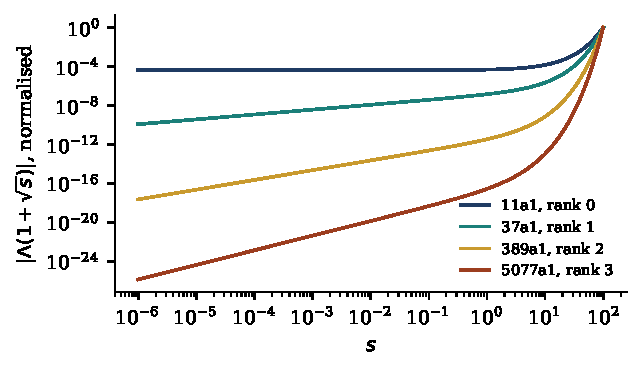
\includegraphics[width=\textwidth]{figs/thorin_rankatom.pdf}
\caption{$|\Lambda(1+\sqrt s,E)|$ on log log axes, normalised to $1$ at $s=100$, for the elliptic curves 11a1, 37a1, 389a1, 5077a1 of ranks $r=0$ to $3$. Near $s=0$ the slopes are $0$, $0.500$, $1.000$, $1.500$: a degenerate Thorin atom of mass $r/2$ at the origin.}\label{fig:10brankatom}
\end{minipage}\hfill
\begin{minipage}[t]{0.48\textwidth}\centering
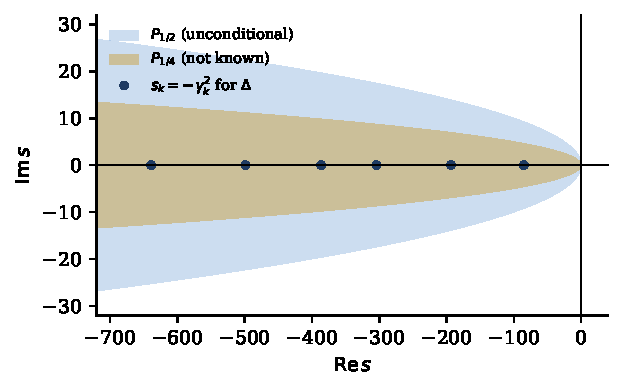
\includegraphics[width=\textwidth]{figs/thorin_parabola10b.pdf}
\caption{The parabolic regions $P_{1/2}$ and $P_{1/4}$ in the plane of $s = z^2$, with the points $s_k = -\gamma_k^2$ for the first six zeros of $\Delta$. For every $\pi$ all $s_k$ lie in $P_{1/2}$ (condition $\Theta_{1/2}$, unconditional); $\Theta_{1/4}$ is known for no $\pi$. GRH puts every $s_k$ on $P_0 = (-\infty,0]$.}\label{fig:10bparabola}
\end{minipage}
\end{figure}

\begin{proposition}[this book]\label{prop:10brank}
Let $\pi\cong\tilde\pi$ with $r = \operatorname{ord}_{s=1/2}\Lambda(s,\pi)\ge1$ and $H(z) = \Lambda(\frac12+z,\pi)/z^r$. Unconditionally,
\[
\lim_{s\to0^+}\frac{d\log|\Lambda(\frac12+\sqrt s,\pi)|}{d\log s} = \frac r2 .
\]
Under GRH for $\pi$, for $s>0$,
\[
\frac{H(0)}{\Lambda(\frac12+\sqrt s,\pi)} = s^{-r/2}\,\E e^{-sX} = \int_0^\infty e^{-sx}\,(m_r*\mu_X)(dx),
\]
with $m_r(dx) = x^{r/2-1}dx/\Gamma(r/2)$, $X$ the GGC of Theorem~\ref{thm:10bmain}(c) for $\Xi^{\mathrm{sd}}_\pi$ and $\mu_X$ its law. The infinite measure $m_r$ is the increasing limit as $\epsilon\downarrow0$ of $\epsilon^{-r/2}$ times the gamma law of shape $r/2$ and rate $\epsilon$, whose Thorin measure is $\frac r2\delta_\epsilon$: a Thorin atom of mass $r/2$ escaping to the origin.
\end{proposition}

\begin{proof}
$\log|\Lambda(\frac12+\sqrt s)| = \frac r2\log s+\log|H(\sqrt s)|$ and $H(\sqrt s)\to H(0)\ne0$ with derivative in $\log s$ tending to zero, which gives the slope. Under GRH, Theorem~\ref{thm:10bmain} gives $H(0)/H(\sqrt s) = \E e^{-sX}$. Also $\int_0^\infty e^{-sx}x^{r/2-1}dx/\Gamma(r/2) = s^{-r/2}$, and the Laplace transform of a convolution of positive measures is the product, by Tonelli. Finally the gamma density of shape $r/2$ and rate $\epsilon$ times $\epsilon^{-r/2}$ is $x^{r/2-1}e^{-\epsilon x}/\Gamma(r/2)$, which increases to the density of $m_r$, and its transform $\epsilon^{-r/2}(1+s/\epsilon)^{-r/2} = (\epsilon+s)^{-r/2}$ tends to $s^{-r/2}$.
\end{proof}

For $r=2$ the density of $m_2*\mu_X$ is $\Prob(X\le x)$. In the product completion $\Xi_\pi$ the central zero has order $2r$ and the degenerate mass is $r$. For an elliptic curve $E/\Q$ the conjecture of Birch and Swinnerton Dyer \cite{bsd1965} identifies the analytic rank with the Mordell Weil rank, so under that conjecture \emph{twice the Thorin mass at the origin of $\Xi^{\mathrm{sd}}$ is the Mordell Weil rank}; for analytic rank at most one this equality is a theorem of Gross and Zagier \cite{grosszagier1986} and Kolyvagin \cite{kolyvagin1988}.\index{Thorin atom at zero}\index{Birch and Swinnerton Dyer conjecture}

Figure~\ref{fig:10brankatom} shows the effect for four curves in the classical normalisation with centre $1$: the slopes of $\log|\Lambda(1+\sqrt s)|$ against $\log s$ between $s = 10^{-6}$ and $10^{-4}$ are $0.500$, $1.000$, $1.500$ for ranks $1$, $2$, $3$ and $0$ for rank $0$, until the atoms $\gamma_k^2$ take over near $s\approx\gamma_1^2$ ($8.27$ for 389a1, $4.21$ for 5077a1).

\section{Parabolic Thorin conditions and the heat flow}\label{sec:10bparabola}

GRH asks that every Thorin atom lie on the half line. A quantitative relaxation asks that they lie in a region around it.

\begin{definition}\label{def:10btheta}
For $\sigma\ge0$, condition $\Theta_\sigma$ for $\pi$ is: every zero $z$ of $\Xi_\pi$ satisfies $|\operatorname{Re}z|\le\sigma$; equivalently every zero of $\Lambda(s,\pi)$ lies in $|\operatorname{Re}s-\frac12|\le\sigma$. Let $P_\sigma = \{x+iy:x\le\sigma^2-y^2/(4\sigma^2)\}$ for $\sigma>0$ and $P_0 = (-\infty,0]$.\index{parabolic Thorin condition}
\end{definition}

\begin{lemma}\label{lem:10bparabola}
For $\sigma\ge0$, $\{z^2:|\operatorname{Re}z|\le\sigma\} = P_\sigma$. Hence $\Theta_\sigma$ holds if and only if every $s_k = z_k^2$ lies in $P_\sigma$, if and only if every Thorin atom $t_k$ lies in $-P_\sigma = \{x+iy:x\ge-\sigma^2+y^2/(4\sigma^2)\}$, the region bounded by the parabola with vertex $-\sigma^2$ that opens along the positive axis. The regions increase with $\sigma$ and $\bigcap_{\sigma>0}(-P_\sigma) = [0,\infty)$.
\end{lemma}

\begin{proof}
The case $\sigma=0$ is $\{(ib)^2\} = (-\infty,0]$. Let $\sigma>0$. The two square roots $\pm w$ of $s = x+iy$ have $|\operatorname{Re}w| = ((|s|+x)/2)^{1/2}$, so $s$ is a square of some $z$ with $|\operatorname{Re}z|\le\sigma$ if and only if $|s|\le2\sigma^2-x$. This requires $x\le2\sigma^2$, and then squaring gives $x^2+y^2\le4\sigma^4-4\sigma^2x+x^2$, that is $x\le\sigma^2-y^2/(4\sigma^2)$; conversely this inequality implies $x\le\sigma^2\le2\sigma^2$. The remaining statements are immediate.
\end{proof}

By Lemma~\ref{lem:10bcompletion}(iii), $\Theta_{1/2}$ holds unconditionally for every $\pi$, with strict inequality: all atoms lie in the interior of $-P_{1/2}$. The image under $z\mapsto z^2$ of the boundary line $\operatorname{Re}z=\frac12$ is the parabola $x = \frac14-y^2$, which is how the nonvanishing theorem of Jacquet and Shalika looks in the $s$ plane. Zero free regions of de la Vall\'ee Poussin type \cite{iwanieckowalski2004} narrow the strip in the $z$ plane by a logarithmically small amount, which in the $s$ plane is a band whose horizontal width grows like $y^2/\log|y|$ (Exercise~\ref{ex:10bzerofree}), but they give $\Theta_\sigma$ for no $\sigma<\frac12$, and for no automorphic $L$ function is $\Theta_\sigma$ known with $\sigma<\frac12$. Condition $\Theta_0$ is GRH (Figure~\ref{fig:10bparabola}).

\subsection{Gaussian tilting}

The P\'olya kernel of Lemma~\ref{lem:10bkernel} can be tilted by a Gaussian factor. For $\lambda\in\R$ put
\[
H_{\pi,\lambda}(t) = \int_{-\infty}^\infty e^{\lambda u^2}\Phi_\pi(u)e^{itu}\,du,
\]
an entire function of $t$, with $H_{\pi,0}(t) = \Xi_\pi(it)/\Xi_\pi(0)$, so $\Theta_\sigma$ says exactly that the zeros of $H_{\pi,0}$ lie in $|\operatorname{Im}t|\le\sigma$. We use de Bruijn's theorem \cite{debruijn1950} in the following form: if $\Phi$ is real, even and integrable with $\Phi(u) = O(\exp(-|u|^{2+\delta}))$ for some $\delta>0$, and all zeros of $H_0(t) = \int\Phi(u)e^{itu}du$ lie in $|\operatorname{Im}t|\le b_0$, then for $\lambda>0$ all zeros of $H_\lambda(t) = \int e^{\lambda u^2}\Phi(u)e^{itu}du$ lie in $|\operatorname{Im}t|\le(\max(b_0^2-2\lambda,0))^{1/2}$. Positivity of $\Phi$ is not needed; see \cite{debruijn1950,newman1976} for the precise hypotheses. By Lemma~\ref{lem:10bkernel} they hold for every $\Phi_\pi$, in particular for $\Delta$ and every multiplicative eta product, and P\'olya's kernel for $\zeta$ satisfies them as well (Chapter~\ref{ch:10}).\index{de Bruijn Newman constant}

\begin{theorem}[Gaussian tilting; (i) de Bruijn, (ii) this book]\label{thm:10btilting}
Suppose $\Theta_\sigma$ holds for $\pi$, and let $\lambda\ge0$.
\begin{enumerate}
\item[(i)] The zeros of $H_{\pi,\lambda}$ lie in $|\operatorname{Im}t|\le\sigma_\lambda$, where $\sigma_\lambda = (\max(\sigma^2-2\lambda,0))^{1/2}$; Gaussian tilting moves the Thorin atoms from $-P_\sigma$ into $-P_{\sigma_\lambda}$, and for $\lambda\ge\sigma^2/2$ all zeros of $H_{\pi,\lambda}$ are real.
\item[(ii)] If $\Phi_\pi\ge0$, let $W_{\pi,\lambda}$ have density proportional to $e^{\lambda u^2}\Phi_\pi(u)$. For every $\lambda\ge\sigma^2/2$ the function $s\mapsto H_{\pi,\lambda}(0)/H_{\pi,\lambda}(i\sqrt s) = 1/\E e^{\sqrt sW_{\pi,\lambda}}$ is the Laplace transform of a GGC with drift zero and Thorin measure $\sum_k\delta_{x_k(\lambda)^2}$, where $\pm x_k(\lambda)$ are the real zeros of $H_{\pi,\lambda}$.
\end{enumerate}
Unconditionally ($\sigma=\frac12$), $H_{\pi,\lambda}$ has only real zeros for every $\lambda\ge\frac18$, and (ii) holds for these $\lambda$.
\end{theorem}

\begin{proof}
(i) is de Bruijn's theorem with $b_0 = \sigma$, translated by Lemma~\ref{lem:10bparabola}. For (ii), $E_\lambda(z) = H_{\pi,\lambda}(-iz)/H_{\pi,\lambda}(0) = \E e^{zW_{\pi,\lambda}}$ is well defined because $H_{\pi,\lambda}(0) = \int e^{\lambda u^2}\Phi_\pi>0$, even because $\Phi_\pi$ is even, real on $\R$, and $E_\lambda(0)=1$. Its order is at most one: with $|\Phi_\pi(u)|\le C\exp(-ce^{c|u|})$ one has $\sup_u(\lambda u^2+|z||u|-\frac c2e^{c|u|}) = O(|z|\log(|z|+2))$. By (i) its zeros $z = ix_k(\lambda)$ lie on $i\R$, so Theorem~\ref{thm:10babstract}, (a) implies (c), applies with $\sigma_0=0$. The unconditional case is $\sigma=\frac12$, from Lemma~\ref{lem:10bcompletion}(iii).
\end{proof}

\begin{remark}[The factor four]
The literature normalisation for $\zeta$ (Chapter~\ref{ch:10}) is $H^{\mathrm{cl}}_0(x) = \frac18\Xi(x/2)$, $\Xi(t) = \xi(\frac12+it)$, with kernel tilt $e^{\lambda_{\mathrm{cl}}v^2}$. Since $t = x/2$, the kernel variables satisfy $u = 2v$, so $e^{\lambda_{\mathrm{cl}}v^2} = e^{(\lambda_{\mathrm{cl}}/4)u^2}$ and $\lambda = \lambda_{\mathrm{cl}}/4$. De Bruijn's classical bound $\lambda_{\mathrm{cl}}\ge\frac12$, from zeros of $H^{\mathrm{cl}}_0$ in $|\operatorname{Im}x|<1$, is our $\lambda\ge\frac18$, from zeros of $H_0$ in $|\operatorname{Im}t|<\frac12$; the Polymath bound $\Lambda\le0.22$ \cite{polymath2019} is $0.055$ in our units.
\end{remark}

Define the de Bruijn Newman constant $\lambda_\pi\in[-\infty,\frac18]$ of $\pi$, in our units, as the infimum of the $\lambda$ for which $H_{\pi,\lambda}$ has only real zeros. If $H_{\pi,\lambda_0}$ has only real zeros, de Bruijn's theorem applied to the kernel $e^{\lambda_0u^2}\Phi_\pi$ with $b_0=0$ shows that $H_{\pi,\lambda}$ has only real zeros for every $\lambda>\lambda_0$. The set of such $\lambda$ is also closed, by Hurwitz's theorem, so it is $[\lambda_\pi,\infty)$ when $\lambda_\pi$ is finite, and GRH for $\pi$ is equivalent to $\lambda_\pi\le0$. When $\Phi_\pi\ge0$, Theorem~\ref{thm:10babstract} (whose equivalence of (a) and (b) needs no strip hypothesis; see the paragraph after its proof) identifies this set with the set of $\lambda$ for which the tilted reciprocal is a GGC transform: \emph{the Thorin property holds exactly on $[\lambda_\pi,\infty)$}. Rodgers and Tao \cite{rodgerstao2020} proved Newman's conjecture $\lambda_\zeta\ge0$, and Dobner's extension \cite{dobner2021} to the extended Selberg class gives $\lambda_\Delta\ge0$, as Chapter~\ref{ch:10} explains; we expect, but do not verify here, that it gives $\lambda_\pi\ge0$ for the other kernels $\Phi_\pi$ of this chapter. For $\zeta$, and for every $\pi$ with $\Phi_\pi\ge0$ and $\lambda_\pi\ge0$, GRH would therefore mean $\lambda_\pi=0$: the tilted reciprocal is a GGC transform for every $\lambda\ge0$ and for no $\lambda<0$. \emph{For such $\pi$, if GRH holds, $1/F_\pi$ lies exactly on the edge of the class of GGC transforms along the heat flow}, in line with Newman's remark that the Riemann hypothesis, if true, is only barely so.

\begin{proposition}[Motion of Thorin atoms]\label{prop:10bflow}
Let $I$ be an open interval of $\lambda$ on which $H_{\pi,\lambda}(0)\ne0$ and all zeros of $H_{\pi,\lambda}$ are real and simple, written $\pm x_k(\lambda)$, $x_k>0$, and let $t_k(\lambda) = x_k(\lambda)^2$. Then each $t_k$ is real analytic on $I$ and
\[
\frac{dt_k}{d\lambda} = 2+8\sum_{j\ne k}\frac{t_k}{t_k-t_j},
\]
the series converging absolutely.
\end{proposition}

\begin{proof}
$H(t,\lambda) = H_{\pi,\lambda}(t)$ is jointly analytic, and differentiating under the integral gives $\partial_\lambda H = -\partial_t^2H$. At a simple zero the implicit function theorem gives analytic $x_k(\lambda)$ with $x_k' = -\partial_\lambda H/\partial_tH = H''(x_k)/H'(x_k)$, primes on $H$ denoting $t$ derivatives. As in the proof of Theorem~\ref{thm:10btilting}, $H_{\pi,\lambda}(t) = H_{\pi,\lambda}(0)(1-t^2/t_k)g(t)$ with $g(t) = \prod_{j\ne k}(1-t^2/t_j)$, locally uniformly convergent. Writing $H = (t-x_k)q(t)$ with $q(t) = -H_{\pi,\lambda}(0)t_k^{-1}(t+x_k)g(t)$ and $q(x_k)\ne0$, we get $H'(x_k) = q(x_k)$ and $H''(x_k) = 2q'(x_k)$, and $g'/g(t) = \sum_{j\ne k}2t/(t^2-t_j)$, so
\[
x_k' = 2\Bigl(\frac1{2x_k}+\sum_{j\ne k}\frac{2x_k}{x_k^2-x_j^2}\Bigr).
\]
Multiplying by $2x_k$ gives the formula. Absolute convergence follows from $|t_k/(t_k-t_j)|\le2t_k/t_j$ for large $j$ and $\sum_jt_j^{-1}<\infty$.
\end{proof}

The constant $2$ is the repulsion of each zero from its mirror image. In the variable $x$ the flow is the classical zero dynamics of the backward heat equation, $x_k' = 2\sum(x_k-x)^{-1}$ over all other zeros $x$, summed symmetrically, and formally $x_k'' = -8\sum(x_k-x)^{-3}$, an inverse cube interaction of Calogero Moser type; the proposition only rewrites it for the Thorin atoms $t_k = x_k^2$. As $\lambda$ decreases the atoms attract; heuristically, a collision is the moment two real zeros meet and leave the axis as a conjugate pair, and $\lambda_\pi$ is the supremum of the collision times. Csordas, Smith and Varga \cite{csordassmithvarga1994} obtained lower bounds for $\lambda_\zeta$ from close pairs of zeros along these lines. We use the dynamics only heuristically; continuation through collisions is not addressed.

\section{A catalogue of applications}

The proof of Theorem~\ref{thm:10bmain} uses only that $\Lambda$ is entire of order one, satisfies a functional equation relating it to its conjugate, and is zero free off the strip $0<\operatorname{Re}s<1$. This is known in the following cases.\index{automorphic $L$ function}

\emph{Dirichlet $L$ functions.} For primitive $\chi\ne1$, $\Lambda(s,\chi)$ is entire; real $\chi$ are self dual, and for complex $\chi$, $\Xi_\chi(x) = |\Lambda(\frac12+x,\chi)|^2/x^{2r}$ on $\R$.

\emph{Dedekind and Hecke $L$ functions.} For a number field $K$, $s(s-1)\Lambda_K(s)$ is entire and symmetric under $s\mapsto1-s$; Hecke $L$ functions of nontrivial Gr\"o{\ss}encharaktere are entire \cite{hecke1918,tate1967}.

\emph{Newforms and elliptic curves.} For a holomorphic newform $f$, $\Lambda(s,f)$ is entire \cite{hecke1937,atkinlehner1970}; by modularity \cite{wiles1995,taylorwiles1995,bcdt2001} this covers every elliptic curve over $\Q$.

\emph{Symmetric powers.} Newton and Thorne \cite{newtonthorne2021,newtonthorne2021b} proved that for every holomorphic newform $f$ of weight at least two without complex multiplication, $\Sym^m\pi_f$ is a cuspidal automorphic representation of $\GL_{m+1}(\A_\Q)$ for every $m\ge1$. Hence Theorem~\ref{thm:10bmain} applies to every symmetric power of every such form. (With complex multiplication $\Sym^mf$ splits into Hecke characters, and for $4\mid m$ a trivial constituent gives a pole, removed as for $\zeta$.)

\emph{Rankin Selberg $L$ functions.} For cuspidal $\pi,\pi'$ with $\pi'\not\cong\tilde\pi$, $\Lambda(s,\pi\times\pi')$ is entire with a functional equation \cite{jpss1983,moeglinwaldspurger1989}, bounded in vertical strips away from the real axis by Gelbart and Shahidi \cite{gelbartshahidi2001}, which gives order one, and nonzero on $\operatorname{Re}s=1$ by Shahidi \cite{shahidi1981}. For $\pi' = \tilde\pi$ there are simple poles at $s=0,1$, removed by the factor $s(s-1)$. Theorem~\ref{thm:10babstract} applies with the same proof.

\emph{Artin $L$ functions.} The theorem applies to every irreducible $\rho$ for which Artin's conjecture is known. By Khare and Wintenberger \cite{kharewintenberger2009} every odd irreducible two dimensional $\rho$ comes from a weight one newform, so this includes all of them. Our example is the representation of $S_3$ cut out by $x^3-x-1$, of conductor $23$, with $L$ function $\zeta_K(s)/\zeta(s)$ for the cubic field $K$, the $L$ function of $\eta(\tau)\eta(23\tau)$.

\begin{table}[t]
\centering
\footnotesize
\setlength{\tabcolsep}{3.2pt}
\begin{tabular}{lrrrrrrrc}
\toprule
$L$ function & $d$ & $N$ & $r$ & $\gamma_1$ & $S_1$ Taylor & $S_1$ zeros & err$(25)$ & Hankel\\
\midrule
$\zeta$ (via $\xi$) & 1 & 1 & 0 & 14.1347 & 0.023105 & 0.023108 & $8.3\cdot10^{-5}$ & yes\\
$L(s,\chi_{-4})$ & 1 & 4 & 0 & 6.0209 & 0.078015 & 0.078013 & $3.9\cdot10^{-5}$ & yes\\
$L(s,\chi_{-3})$ & 1 & 3 & 0 & 8.0397 & 0.056701 & 0.056696 & $1.1\cdot10^{-4}$ & yes\\
$L(s,\chi_5)$ & 1 & 5 & 0 & 6.6485 & 0.078457 & 0.078462 & $1.3\cdot10^{-4}$ & yes\\
$\Delta$ & 2 & 1 & 0 & 9.2224 & 0.0561759 & 0.0561824 & $1.7\cdot10^{-4}$ & yes\\
11a1 & 2 & 11 & 0 & 6.3626 & 0.127589 & 0.127584 & $1.1\cdot10^{-4}$ & yes\\
37a1 & 2 & 37 & 1 & 5.0032 & 0.189609 & 0.189611 & $5.4\cdot10^{-5}$ & yes\\
389a1 & 2 & 389 & 2 & 2.8761 & 0.407048 & 0.407051 & $1.0\cdot10^{-4}$ & yes\\
5077a1 & 2 & 5077 & 3 & 2.0525 & 0.725919 & 0.725921 & $6.0\cdot10^{-5}$ & yes\\
Artin, $x^3-x-1$ & 2 & 23 & 0 & 5.1157 & 0.170287 & 0.170294 & $1.8\cdot10^{-4}$ & yes\\
$\Sym^2$ 11a1 & 3 & 121 & 0 & 3.8993 & 0.321206 & 0.321205 & $2.1\cdot10^{-5}$ & yes\\
\bottomrule
\end{tabular}
\caption{The global Thorin catalogue, computed with $\Xi^{\mathrm{sd}}$: degree $d$, conductor $N$, central order $r$, first ordinate $\gamma_1$ beyond the centre, $S_1 = \sum\gamma_k^{-2}$ from central Taylor coefficients and from the zeros to height $300$ plus the tail estimate, absolute relative error of the product formula at $s=25$, and positivity of $\det(S_{i+j+1})_{m\times m}$, $m\le4$, and $\det(S_{i+j+2})_{m\times m}$, $m\le3$, computed from Taylor coefficients alone.}\label{tab:10bcatalogue}
\end{table}

Table~\ref{tab:10bcatalogue} records computations carried out for this book on eleven self dual $L$ functions, using $\Xi^{\mathrm{sd}}$. We computed the zeros to height $T = 300$ ($138$ to $680$ of them) and compared $\Xi^{\mathrm{sd}}(\sqrt s)/\Xi^{\mathrm{sd}}(0)$ with $\prod(1+s/\gamma_k^2)\exp(s\sum_{\gamma>T}\gamma^{-2})$, the tail estimated by $(\log N+d\log(T/2\pi)+d)/(2\pi T)$, which is the integral of $t^{-2}$ against the zero density $(\log N+d\log(t/2\pi))/(2\pi)$ over $t>T$. The relative error is at most $2.8\cdot10^{-5}$ at $s=4$, $1.8\cdot10^{-4}$ at $s=25$ and $8\cdot10^{-4}$ at $s=100$ in every case. The same tail estimate is added to $S_1$ from zeros in the table. For $S_3$ and $S_4$ the values from Taylor coefficients and from zeros agree to all printed digits, for instance $1.8373\cdot10^{-6}$ and $2.0017\cdot10^{-8}$ for $\Delta$, $1.4417\cdot10^{-7}$ and $6.6303\cdot10^{-10}$ for $\zeta$. For $S_2$ the zero sums carry no tail correction and fall short of the Taylor values ($1.9975\cdot10^{-4}$ for $\Delta$, $3.7173\cdot10^{-5}$ for $\zeta$) by the omitted tail $\sum_{\gamma>T}\gamma^{-4}$, a relative amount of at most $2.2\cdot10^{-4}$. The coefficients of $\log F(s)$ alternate in sign through $n=8$ for all eleven functions, as GRH requires (Remark~\ref{rem:10bfinite}). The Hankel determinants $\det(S_{i+j+1})_{m\times m}$, $m\le4$, and $\det(S_{i+j+2})_{m\times m}$, $m\le3$, computed from central Taylor coefficients at $60$ digit precision without using any zero, are positive in every case; for $\Delta$ the first family is $5.618\cdot10^{-2}$, $6.331\cdot10^{-8}$, $4.749\cdot10^{-19}$, $9.579\cdot10^{-36}$, and for $\zeta$ it is $2.310\cdot10^{-2}$, $1.949\cdot10^{-9}$, $2.173\cdot10^{-22}$, $1.178\cdot10^{-41}$. These are necessary conditions for GRH, so the computation is consistent with it; by Remark~\ref{rem:10bfinite} it constrains only the lowest atoms.

\section{The Thorin threshold}

Everything above requires $\sum_k|t_k|^{-1}<\infty$, which makes $F$ a genus zero product and $\sum E_k/t_k$ convergent; for automorphic $L$ functions $N(T)\asymp T\log T$ gives it with room to spare. The Selberg zeta function crosses this threshold.\index{Thorin threshold}

Let $\Gamma\backslash\mathbb H$ be a compact hyperbolic surface with Laplace eigenvalues $0 = \lambda_0<\lambda_1\le\lambda_2\le\dots$ and write $\lambda_j = \frac14+r_j^2$. Selberg's zeta function $Z_\Gamma(s)$ \cite{selberg1956,hejhal1976} has zeros at $s = \frac12\pm ir_j$, and by Sarnak \cite{sarnak1987b} it equals, up to an explicit factor built from the Barnes double gamma function, the regularised determinant $\det(\Delta_\Gamma-s(1-s))$. Removing the zeros at $s=0,1$ from $\lambda_0 = 0$ and assuming for simplicity that $\frac14$ is not an eigenvalue, we obtain an even entire $E_\Gamma(z)$, real on $\R$, $E_\Gamma(0) = 1$, with zeros $\pm ir_j$, $j\ge1$, and put $F_\Gamma(s) = E_\Gamma(\sqrt s)$. Its Thorin atoms are
\[
t_j = r_j^2 = \lambda_j-\tfrac14,
\]
the spectrum of $\Delta_\Gamma-\frac14$. But Weyl's law $\#\{j:\lambda_j\le x\}\sim\frac{\operatorname{area}}{4\pi}x$ \cite{weyl1912,hejhal1976} gives $\#\{j:|r_j|\le T\}\sim\frac{\operatorname{area}}{4\pi}T^2$, so $E_\Gamma$ has order two, $\sum_j|t_j|^{-1}$ diverges logarithmically and $\sum_j|t_j|^{-2}<\infty$. The reciprocal is no longer a GGC transform even when all $t_j>0$, but a compensated version survives.

\begin{proposition}[Regularised Thorin equivalence; this book]\label{prop:10bregularised}
Let $E$ be entire, even, real on $\R$, $E(0)=1$, of order at most two with zeros $\pm z_k$ satisfying $\sum|z_k|^{-4}<\infty$, and let $t_k = -z_k^2$, $F(s) = E(\sqrt s)$. Then $F(s) = e^{bs}\prod_k(1+s/t_k)e^{-s/t_k}$ for some real $b$, and the following are equivalent: (a) all $t_k>0$; (b) for independent standard exponential variables $E_k$ the series $Y = b+\sum_k(E_k-1)/t_k$, which converges in $L^2$, is real valued and satisfies $1/F(s) = \E e^{-sY}$ for $s\ge0$; (c) $1/F$ agrees on $(0,\infty)$ with a function holomorphic and zero free on $\C\setminus(-\infty,0]$. The law of $Y$ in (b) is infinitely divisible with L\'evy measure $x^{-1}\sum_ke^{-t_kx}dx$ on $(0,\infty)$; when $\sum_kt_k^{-1} = \infty$ its first moment $\int_0^1\sum_ke^{-t_kx}dx$ near the origin is infinite, which is why the centring is needed.
\end{proposition}

\begin{proof}
$F$ has order at most one with $\sum|t_k|^{-2}<\infty$, so Hadamard's theorem gives the genus one product with a factor $e^{a+bs}$, $a = 0$ since $F(0)=1$; $b$ is real since $\{t_k\}$ is closed under conjugation and $F$ is real on $(0,\infty)$. The series for $Y$ converges in $L^2$ because its summands are independent with mean zero and $\sum_k|t_k|^{-2}<\infty$. (a) implies (b): if all $t_k>0$ the series also converges almost surely, and $\E e^{-s(E_k-1)/t_k} = e^{s/t_k}(1+s/t_k)^{-1}$. For fixed $s\ge0$ the normalised partial products $e^{-sY_N}/\E e^{-sY_N}$, with $Y_N = \sum_{k\le N}(E_k-1)/t_k$, form a positive martingale whose second moments are $\prod_{k\le N}(1+s/t_k)^2(1+2s/t_k)^{-1}\le\prod_k(1+s^2/t_k^2)<\infty$; it is therefore uniformly integrable, and passing to the limit gives (b). (b) implies (a): the imaginary part of $Y$ is $\sum_k\operatorname{Im}(t_k^{-1})(E_k-1)$, a sum of independent variables that has a continuous law as soon as one coefficient is nonzero, so $Y$ real forces every $t_k$ real; and a real $t_k<0$ would make $\E e^{-s(E_k-1)/t_k}$, hence $\E e^{-sY}$, infinite for every $s\ge|t_k|$, while $1/F$ is finite on $(0,\infty)$ outside a discrete set. (a) implies (c): each factor $e^{s/t_k}(1+s/t_k)^{-1}$ is holomorphic and zero free on $\C\setminus(-\infty,0]$ and the product converges locally uniformly there. (c) implies (a): the identity theorem shows that $F$ has no zeros off $(-\infty,0]$, and $F(0) = 1$, so all $t_k>0$. The L\'evy measure follows from Frullani's integral applied to each factor.
\end{proof}

For the surface, (a) says $\lambda_1\ge\frac14$ (strictly, under our simplifying assumption): the Thorin property of the regularised reciprocal of the Selberg zeta function is the absence of exceptional eigenvalues. On a general surface small eigenvalues give negative atoms $t_j\in(-\frac14,0)$. For arithmetic surfaces this is Selberg's eigenvalue conjecture \cite{selberg1965}, for congruence subgroups of $\SL_2(\Z)$ and, through the Jacquet Langlands correspondence \cite{jacquetlanglands1970}, for the compact quaternion surfaces over $\Q$. There the bound $\lambda_1\ge\frac{975}{4096} = \frac14-(\frac7{64})^2$ of Kim and Sarnak \cite{kimsarnak2003} says precisely that every atom satisfies $t_j\ge-(\frac7{64})^2$: condition $\Theta_{7/64}$ for the spectral zeros. (For noncompact congruence surfaces the zeros from the scattering determinant must first be separated.) In field theoretic terms, if all $t_j>0$ then $\sum_jE_j/t_j$ is the formal squared norm of the complex Gaussian field with covariance $(\Delta_\Gamma-\frac14)^{-1}$, and the centring in $Y$ is its Wick renormalisation, needed because that norm diverges logarithmically in two dimensions.

\begin{problem}[Selberg's conjecture as a regularised Thorin problem]
For the family of compact arithmetic surfaces attached to maximal orders in indefinite quaternion algebras over $\Q$, or for congruence surfaces after removal of the scattering zeros, construct directly, without spectral input and uniformly in the level, real random variables $Y_\Gamma$ with $\E e^{-sY_\Gamma} = 1/F_\Gamma(s)$ for every $s\ge0$; under (a) of Proposition~\ref{prop:10bregularised} the variable of its part (b) is one. Since the atoms $t_j = \lambda_j-\frac14$ are real, a negative atom would make $1/F_\Gamma$ infinite at the point $s = -t_j>0$ but finite at $0$ and at all large $s$, which is impossible for a Laplace transform, whose domain of finiteness is an interval. Such a construction would therefore prove Selberg's eigenvalue conjecture for the family. More modestly, develop the Thorin theory of order two: the analogues of the L\'evy function criterion and of the Hankel criterion, Theorem~\ref{thm:10babstract}(d) and (f), for compensated sums.
\end{problem}

\section{Pictures of the Thorin property}
Figures~\ref{fig:10bphase} and \ref{fig:10bthorin} show the two sides of Theorem~\ref{thm:10bmain} for $\Delta$. The phase portrait of $\Lambda(6+z,\Delta)$ (classical normalisation, centre $6$) colours each point by the argument of the function, with brightness bands for its modulus; a zero is a point where every colour meets. In the window every zero lies on the axis $\mathrm{Re}\,z=0$, as the Riemann hypothesis for $\Delta$ predicts; this is a numerical observation, not a proof. Since $\Lambda(6+z,\Delta)$ is even in $z$, the reciprocal $\Lambda(6)/\Lambda(6+\sqrt s)$ is meromorphic in the whole plane of $s=z^2$, and in the window its only poles are the points $-\gamma_k^2$ on the negative axis: this is the analytic shape of a generalized gamma convolution whose Thorin measure is $\sum_k\delta_{\gamma_k^2}$.

\begin{figure}[ht]\centering
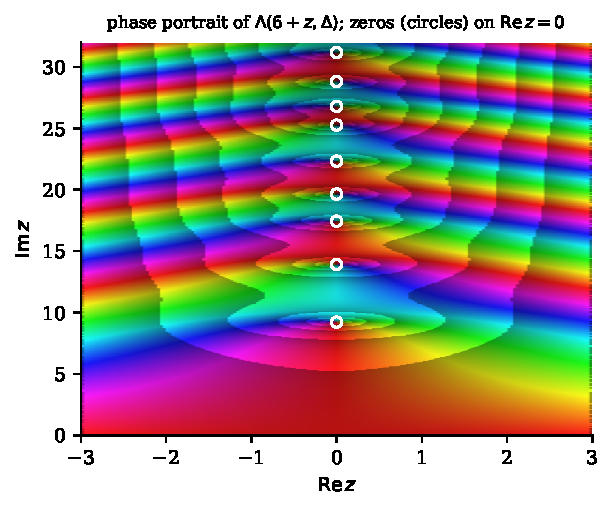
\includegraphics[width=0.92\textwidth]{figs/domain_delta.pdf}
\caption{Phase portrait of $\Lambda(6+z,\Delta)$ for $|\mathrm{Re}\,z|\le3$, $0\le\mathrm{Im}\,z\le32$, with the modulus normalised along each horizontal line. The white circles mark the zeros found on $\mathrm{Re}\,z=0$ by PARI/GP; the colours show no other zero in the window.}\label{fig:10bphase}
\end{figure}

\begin{figure}[ht]\centering
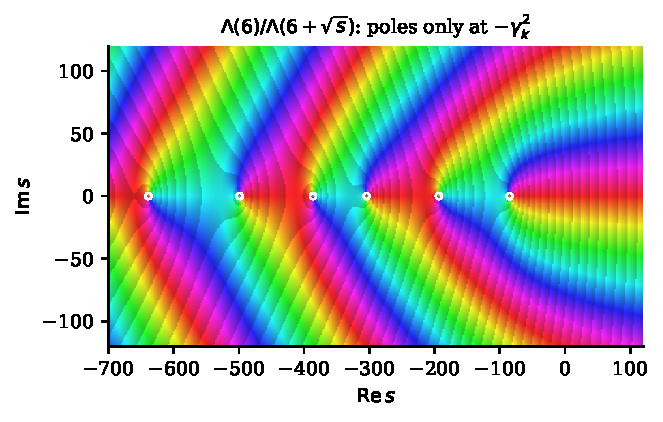
\includegraphics[width=0.95\textwidth]{figs/domain_thorin.pdf}
\caption{Domain colouring of $\Lambda(6,\Delta)/\Lambda(6+\sqrt s,\Delta)$ in the $s$ plane. The circles mark $-\gamma_k^2$ for the first six zeros of $\Delta$; the colour wheel winds around each of them with the orientation of a pole, and around no other point of the window.}\label{fig:10bthorin}
\end{figure}

\section{Notes}

For generalized gamma convolutions, the reciprocal $\Xi$ function, the Brownian reading of $\xi$ and the heat flow see the Notes to Chapter~\ref{ch:10}. Bernstein's theorem is \cite{bernstein1929}; Stieltjes functions and their Nevanlinna Pick characterisation are treated in \cite{schillingsongvondracek2012}, and the moment problem on the half line in \cite{stieltjes1894,akhiezer1965}. The equivalence of (a), (b) and (c) of Theorem~\ref{thm:10babstract} for Laguerre P\'olya functions, with its van Dantzig and Wald forms, is from \cite{polson2018vdp}. As far as we know, the self dual completion for general $\pi$, the forms (d), (e) and (f) in this generality, the cumulant criterion, the rank atom, the parabolic and tilted versions and the computations have not appeared in this form, although each rests on classical ingredients: Hankel criteria for real zeros go back to Hermite and Grommer \cite{grommer1914}, and Newton's identities link the power sums $S_n$ to the central Taylor coefficients. The results labelled as ours are elementary consequences of Hadamard's factorisation, the identity theorem and the classical facts cited; none proves a Riemann hypothesis. The zero dynamics under the heat flow, which Proposition~\ref{prop:10bflow} rewrites for the Thorin atoms, were used by Csordas, Smith and Varga \cite{csordassmithvarga1994} and by the Polymath project \cite{polymath2019}. Numerical values were computed for this book with PARI/GP \cite{pari2023}; the first zeros agree with those listed in the LMFDB \cite{lmfdb}.

\section{Exercises}

\begin{enumerate}
\item Let $g(s) = \sum_{j=1}^Jc_j/(s+t_j)$ with $c_j>0$ and distinct real $t_j$. Show directly that $\operatorname{Im}g(s)\le0$ on the upper half plane, and that $g$ is a Stieltjes function if and only if every $t_j\ge0$. Show that if the $t_j$ may be complex, closed under conjugation with equal weights on conjugate pairs, then $\operatorname{Im}g\le0$ on the upper half plane forces all $t_j$ real.
\item For $\nu>-1$ let $E_\nu(z) = \Gamma(\nu+1)(2/z)^\nu I_\nu(z)$, whose zeros are $\pm ij_{\nu,k}$ with $j_{\nu,k}>0$ the zeros of $J_\nu$. Show that $E_\nu$ satisfies the hypotheses of Theorem~\ref{thm:10babstract}, that $S_1 = \frac1{4(\nu+1)}$ and $S_2 = \frac1{16(\nu+1)^2(\nu+2)}$, and check the case $\nu = \frac12$, $E(z) = \sinh z/z$, against $\sum(\pi k)^{-2} = \frac16$ and $\sum(\pi k)^{-4} = \frac1{90}$. Compute $S_3$ and $S_4$ by Corollary~\ref{cor:10bnewton} and verify that the two $2\times2$ Hankel determinants $S_1S_3-S_2^2$ and $S_2S_4-S_3^2$ are positive.
\item\label{ex:10bzerofree} Verify Lemma~\ref{lem:10bparabola} by showing that $z\mapsto z^2$ maps the line $\operatorname{Re}z = a>0$ onto the parabola $x = a^2-y^2/(4a^2)$. Show that the image of the curve $\operatorname{Re}z = \frac12-c/\log(|\operatorname{Im}z|+3)$ lies at horizontal distance asymptotic to $4cy^2/\log|y|$ from the parabola $x = \frac14-y^2$ as $|y|\to\infty$: a zero free region that is logarithmically thin in the $z$ plane is a wide region in the $s$ plane.
\item Let $E/\Q$ have analytic rank $2$, assume GRH for $E$, and put $H(z) = \Lambda(1+z,E)/z^2$. Show that $H(0)/\Lambda(1+\sqrt s,E) = \int_0^\infty e^{-sx}\Prob(X\le x)\,dx$ with $X$ the GGC of Proposition~\ref{prop:10brank}, and deduce that $s\mapsto H(0)/\Lambda(1+\sqrt s,E)$ is completely monotone on $(0,\infty)$. For rank $3$ find the corresponding fractional integral.
\item Let $W$ be the P\'olya variable of $\zeta$. Using Proposition~\ref{prop:10bcumulants} and $S_1 = 0.023105$, $S_2 = 3.7173\cdot10^{-5}$, compute the variance and the excess kurtosis $\kappa_4/\kappa_2^2 = -3S_2/S_1^2$ of $W$. Prove that $-3S_2/S_1^2\in(-3,0)$ whenever all $t_k>0$ and there are at least two atoms, and show by an example with one conjugate pair of nonreal atoms that $-3S_2/S_1^2$ can then be positive.
\end{enumerate}

\section{Open computational problems}

\begin{compproblem}[Certified Thorin Hankel determinants]
Objective: certify the positivity of the Hankel determinants $\det(S_{i+j+1})_{m\times m}$ and $\det(S_{i+j+2})_{m\times m}$ for $m\le20$, computed from central derivatives only. Objects and scale: all $L$ functions in LMFDB of degree at most $4$ and analytic conductor below $10^3$. Route: central derivatives $\Xi^{(2j)}(0)$, $2j\le80$, in rigorous ball arithmetic (Arb, cross checked with PARI/GP \texttt{lfun}), Corollary~\ref{cor:10bnewton} in interval arithmetic, and interval Cholesky factorisation; the precision needed grows roughly like $m^2\log t_m$ digits. Deliverable: a table of certified lower bounds for the smallest eigenvalue of each Hankel matrix, and the smallest $m$ at which certification fails for lack of precision. Why it matters: these are the finite sections of the Thorin Hankel criterion, Theorem~\ref{thm:10bmain}(f), and the margins quantify how the criterion sees the lowest atoms (Remark~\ref{rem:10bfinite}).
\end{compproblem}

\begin{compproblem}[The Herglotz test in the upper half plane]
Objective: map $\operatorname{Im}(F'/F)(s)$ on a grid in $\{\operatorname{Im}s>0\}$ and measure its distance from violating Theorem~\ref{thm:10bmain}(e). Objects and scale: the eleven functions of Table~\ref{tab:10bcatalogue} and all elliptic curves of conductor below $10^4$, on a logarithmic grid with $\operatorname{Re}s\in[-10^4,10^2]$, $\operatorname{Im}s\in[10^{-3},10^3]$, about $10^6$ points each; on the lines $\operatorname{Im}s=\varepsilon$ the map gives, up to a constant factor and the change of variable $z=-\operatorname{Re}s$, the signed densities $u_\varepsilon$ of Chapter~\ref{ch:scholze}. Route: $\Lambda$ and $\Lambda'$ at $\frac12+\sqrt s$ with PARI/GP \texttt{lfunlambda}, parallelised over grid points. Deliverable: heat maps of $-\operatorname{Im}(F'/F)\cdot|s|$, the minimum over the grid, and an empirical law for how the minimum decays as the grid approaches the negative axis. Why it matters: an off line zero $z_0$ of $\Xi$ would give a pole of $F'/F$ at $s_0 = z_0^2$, with $\operatorname{Im}s_0 = 2|\operatorname{Re}z_0\operatorname{Im}z_0|$, surrounded by a region where $\operatorname{Im}(F'/F)>0$; the computation calibrates how such a region would be seen.
\end{compproblem}

\begin{compproblem}[Collision times of the Thorin atoms of $\Delta$]
Objective: measure how close the low zeros of $\Delta$ are to leaving the critical line under the backward heat flow. Let $\lambda_c(K)<0$ be the first collision time of the truncated system in which the lowest $K$ atoms $\gamma_k^2$ move from $\lambda = 0$ downwards by the equation of Proposition~\ref{prop:10bflow}, the atoms beyond them being replaced in the interaction sum, from $\gamma_{K+1}$ on, by their fixed smooth density $\frac1\pi\log\frac{\gamma}{2\pi}$ in the ordinate $\gamma$; the atoms are those of the self dual kernel $\Phi^{\mathrm{sd}}_\Delta$, since the proposition needs simple zeros and for the product kernel $\Phi^{\mathrm{sd}}_\Delta*\Phi^{\mathrm{sd}}_\Delta$ every atom is double. Objects and scale: $K$ from $10$ to $10^5$, hence the first $10^5$ zeros of $L(s,\Delta)$, and $\lambda\in[-1,0]$. Route: zeros by PARI/GP \texttt{lfunzeros}, an adaptive implicit integrator with fast multipole summation, validated for small $|\lambda|$ against the zeros of $t\mapsto\int e^{\lambda u^2}\Phi^{\mathrm{sd}}_\Delta(u)\cos(tu)\,du$ located by quadrature. Deliverable: $\lambda_c(K)$ on a grid of $K$, the pair responsible (a Lehmer pair for $\Delta$), and the dependence of $\lambda_c(K)$ on $K$. Why it matters: since $\lambda_\Delta\ge0$ (Chapter~\ref{ch:10}), the Riemann hypothesis for $\Delta$ would make the Thorin property hold exactly for $\lambda\ge0$ (Theorem~\ref{thm:10btilting} and the discussion after it) and, heuristically, $0$ the supremum of the collision times; $\lambda_c(K)$ measures how narrowly the hypothesis would hold among the lowest $K$ atoms.
\end{compproblem}

\begin{compproblem}[A regularised Thorin computation for a Selberg zeta function]
Objective: test Proposition~\ref{prop:10bregularised} numerically for an arithmetic surface. Objects and scale: the first $10^4$ Laplace eigenvalues of the compact quotient $\Gamma\backslash\mathbb H$, with $\Gamma$ the norm one units of a maximal order in the quaternion algebra of discriminant $6$ over $\Q$ (an orbifold of genus $0$), and of the modular surface (Maass cusp forms, scattering part separated). Route: eigenvalues by Hejhal's method or finite elements, checked against the trace formula and Weyl's law; the law of $Y = b+\sum_j(E_j-1)/t_j$ by Monte Carlo with $10^6$ draws and the Weyl tail added as a Gaussian correction. Deliverable: the atoms $t_j = \lambda_j-\frac14$, a plot of the L\'evy function $\sum_je^{-t_jx}$ against its Weyl asymptote $\frac{\operatorname{area}}{4\pi x}$ as $x\to0$, and the density of $Y$. Why it matters: it tests the Thorin framework beyond the threshold, where the reformulated conjecture is Selberg's eigenvalue conjecture rather than a Riemann hypothesis.
\end{compproblem}
